\tikzstyle{block} = [draw, fill=blue!20, rectangle, 
    minimum height=3em, minimum width=4em]
\tikzstyle{sum} = [draw, fill=blue!20, circle, node distance=1cm]
\tikzstyle{input} = [coordinate]
\tikzstyle{output} = [coordinate]
\tikzstyle{pinstyle} = [pin edge={to-,thin,black}]


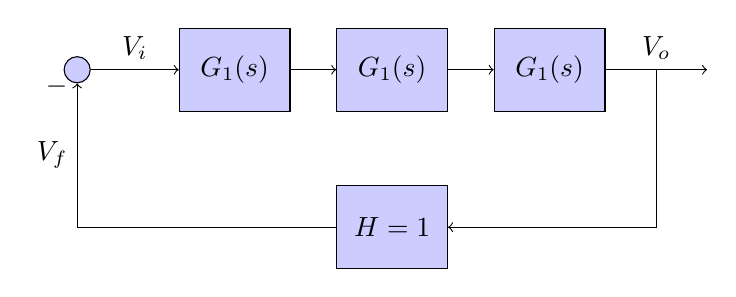
\begin{tikzpicture}[auto, node distance=2cm]
    \node [input, name=input] {};
    \node [sum, right of=input] (sum) {};
    \node [block, right of=sum] (controller1) {$G_1(s)$};
    \node [block, right of=controller1] (controller2) {$G_1(s)$};
    \node [block, right of=controller2] (controller3) {$G_1(s)$};
    \node [output, right of=controller3] (output) {};
    \node [block, below of=controller2] (feedback) {$H = 1$};

    \draw [->] (sum) -- node {$V_i$} (controller1);
    \draw [->] (controller1) -- node {} (controller2);
    \draw [->] (controller2) -- node {} (controller3);
    \draw [->] (controller3) -- node [name=y] {$V_o$}(output);
    \draw [->] (y) |- (feedback);
    \draw [->] (feedback) -| node[pos=0.99]{$-$}  node [near end] {$V_f$} (sum);
\end{tikzpicture}
